\documentclass{beamer}
\usetheme{Madrid}
\usepackage{graphicx}
\usepackage[T1]{fontenc}
\usepackage[polish]{babel}
\usepackage[polish]{datetime2}

\usepackage{tikz}
\def\checkmark{\tikz\fill[scale=0.4](0,.35) -- (.25,0) -- (1,.7) -- (.25,.15) -- cycle;} 


\title{Games classifier}

\author[Team name]{Team name\\[5mm]
{\small Members: Julia Cygan, Borys Adamiak, Patryk Flama}
\hspace{18mm} 
{\small Supervisor: Marek Adamczyk}}

\institute{UWr}
\date{\today}

\begin{document}

\begin{frame}
\titlepage
\end{frame}


\begin{frame}[t]{Your task}

\vspace{-0.5cm}

\begin{columns}
\begin{column}[t]{0.5\textwidth}

{\bf Goal and motivation}

We want to be able to automatically assign tags (or genres) to games, based on their text description. \\
Solution to such problem has real-world applications, such as game grouping/filtering or finding simmilar games or trends analysis. \\
Additionally, in aspect of ML project, we want to make a small comparison of different models and data processing methods for such multilabel classification problem.

\end{column}

\pause

\begin{column}[t]{0.5\textwidth}

{\bf Info about the data}

Steam has its own official API, from which we want to download all of the data (and since Steam is the largest library it will allow for a lot of diverse, high quality, data). \\
Currently there are above 100'000 games, which does create a large dataset. \\
After cleaning the data (removing empty descriptions or tags, removing tags that occur only once) we ended up with a dataset of size around 50'000 games and 400 tags or 100 genres.

\end{column}
\end{columns}

\end{frame}


\begin{frame}[t]{Methods}

Data processing

\begin{itemize}
\item Bag of Words - binary vector records if word appears in text (input representation) \checkmark
\item TF-IDF - term frequency * inverse document frequency (input representation) \checkmark
\item Hashing vectorizer - method to generate low-dimensional input representation (input representation) \checkmark
\item multi label binary vector (output representation) \checkmark

\end{itemize}
\end{frame}

\begin{frame}[t]{Models}

\begin{itemize}
    \item KNN \checkmark
    \item Logistic Regression \checkmark
    \item Decision Trees + Random Forest \checkmark
	\item Naive Bayes \checkmark
	\item Simple perceptron-based neural network \checkmark
	\item Support Vector Machine \checkmark
\end{itemize}
\end{frame}

\begin{frame}[t]{Evaluation}
\only<1-2>{
After analyzing the problem we came to conclusion that evaluaion methods are very interesing and important part of this project.

\pause

\begin{itemize}
	\item We dont want to falsely assign a tag to a game that should not have it
	\item Its more important to assing high percentage of tags to games, than to assign as many as possible
	\begin{itemize}
		\item Game should have 10 tags, but we only assign 8 (not bad)
		\item Game should have 1 tag, but we do not assign any (this is worse) 
	\end{itemize}
\end{itemize}
}

\pause

\begin{itemize}
\item Recall {\it TP/(TP+FN)} - we prefer to have more FN than to have an TP
 \checkmark
\item F1-score {\it (2 * precision * recall) / (precision + recall)} - nice name, but also it combines precision with recall thus both TP and FN are equally expensive \checkmark

\item Hammming loss
\item Intersection over union score
\item Exact match

\end{itemize}


\end{frame}


\begin{frame}[t]{Input data}
\only<1>{First we tried some unsupervised methods to check if we can find some patterns in the data}
	
\centering

\only<2-3>{
	PCA on Bag of Words representation of the data (to 10'000 words) \\
	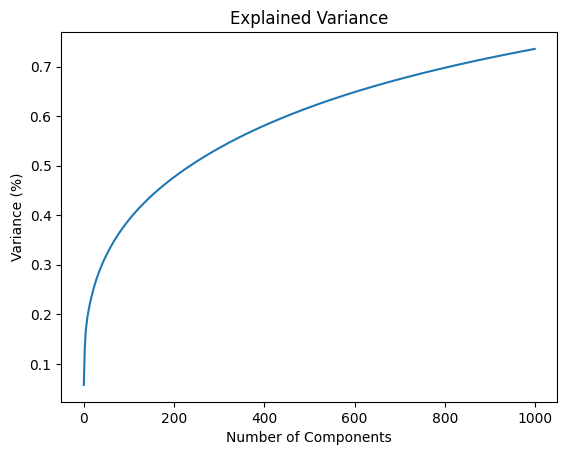
\includegraphics[width=0.6\textwidth,height=0.6\textheight,keepaspectratio]{images/pca_bow.png} % Replace with your image file
	
	\pause
	
	Nice, out of 10'000 dimensions we can create ~100 that 'explain' about half of the data.
}

\only<4-5>{
	t-SNE representation of same data \\
	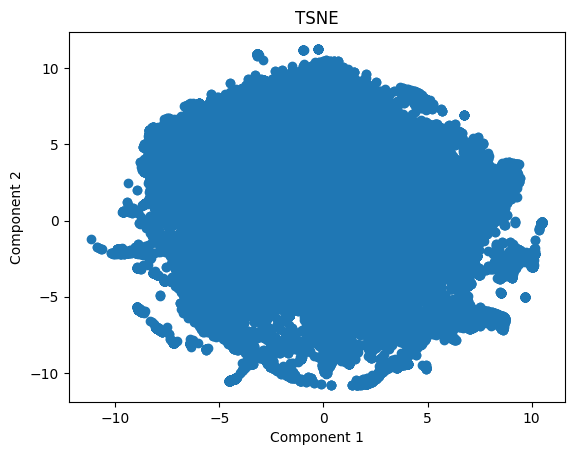
\includegraphics[width=0.6\textwidth,height=0.6\textheight,keepaspectratio]{images/tsne_300_bow.png} % Replace with your image file
	
	\pause
	
	And it does not look that helpful :<
}

\only<5-6>{
	But what about combining PCA with t-SNE?
}

\end{frame}

\end{document}